\section{Présentation des dataset secondaires}

\textbf{Nom du Dataset :} gc\_data.csv

\vspace{0.5cm}
\textbf{Les colonnes du dataset :}
\begin{itemize}
	\item School, Program, Result, Result\_Date, GPA, 
	\item Verbal\_GRE, Quant\_GRE, Writing\_GRE, Subject\_GRE, 
	\item Status, Submit\_Date, Degree\_Type
\end{itemize}

\vspace{0.5cm}
\textbf{Aperçu des 5 premières lignes du dataset :}

\begin{center}
	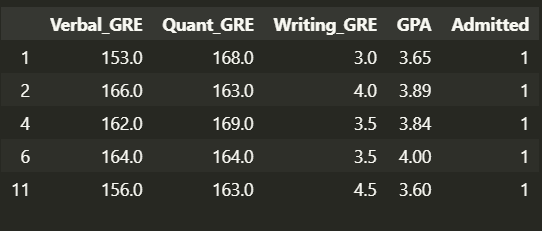
\includegraphics[width=0.9\textwidth]{../figures/head.png}
	\captionof{figure}{Aperçu des 5 premières lignes du dataset}
\end{center}

\begin{center}
	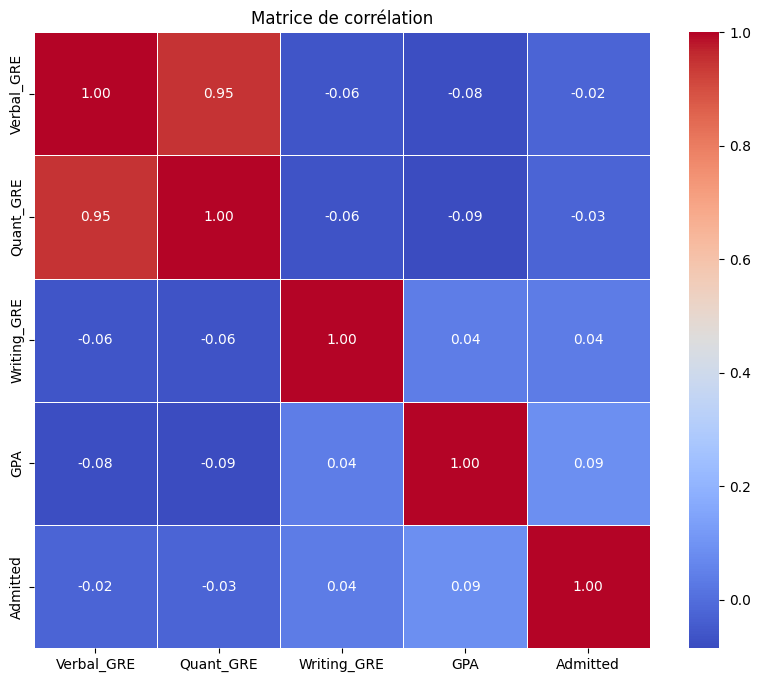
\includegraphics[width=0.9\textwidth]{../figures/corr.png}
\end{center}

Les variables principales du dataset secondaire \textbf{gc\_data.csv} (Verbal\_GRE, Quant\_GRE, Writing\_GRE et GPA) sont faiblement corrélées à la variable cible (\textbf{Admitted}). Cette faiblesse de corrélation peut être due à une falsification des données.

\vspace{0.5cm}
\textbf{Choix des variables explicatives (X) :} \\
Nous avons sélectionné les variables suivantes comme variables explicatives :
\begin{itemize}
	\item Verbal\_GRE
	\item Quant\_GRE
	\item Writing\_GRE
	\item GPA
	\item Admitted
\end{itemize}

\vspace{0.3cm}
\textbf{Variable cible (Y) :} \\
La variable cible est \textbf{Admitted}. Cette variable correspond à notre objectif d'étude, car elle représente la classification binaire : 1 pour admit et 0 pour le contraire, permettant de prédire si l'étudiant peut être admis ou non.

\textbf{Nom du Dataset :} Australian\_Student\_PerformanceData (ASPD24).csv \\
Ce dataset contient des données de performance des étudiants australiens.

\vspace{0.5cm}
\textbf{Les colonnes dans le dataset :}
\begin{itemize}
	\item 51 colonnes, y compris :
	\begin{itemize}
		\item GPA
		\item High School GPA
		\item Entrance Exam Score
		\item Attendance
		\item Family Income
		\item Parental Education
		\item Health
		\item Mental Health
		\item Exam Scores
		\item Final Exam Scores
		\item Gender
		\item Hours of Study per Week
		\item Performance ou P\_encoded après l'encodage de la variable cible
	\end{itemize}
\end{itemize}


\vspace{0.5cm}
\textbf{Aperçu des 5 premières lignes du dataset :}

\begin{center}
	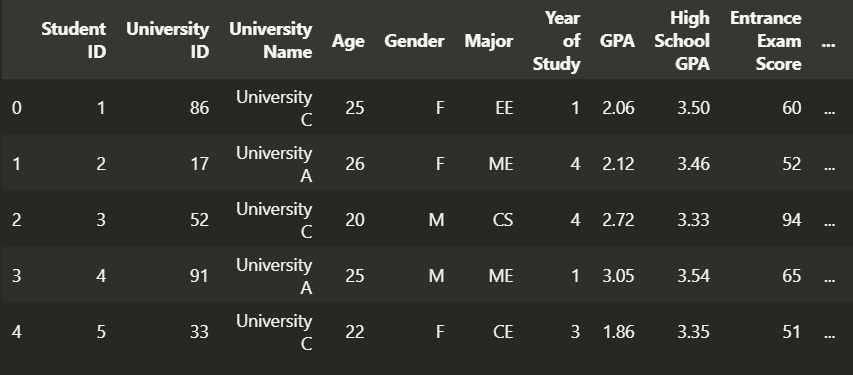
\includegraphics[width=0.9\textwidth]{../figures/head1.png}
	\captionof{figure}{Les 5 premières lignes du dataset}
\end{center}

Les variables indépendantes suivantes : GPA, High School GPA, Entrance Exam Score, Attendance, Family Income, Parental Education, Health, Mental Health, Exam Scores sont peu corrélées à la variable cible (\textbf{Performance} ou \textbf{P\_encoded}), comme le montre la figure ci-dessous.

\begin{figure}[!htbp]
	\centering
	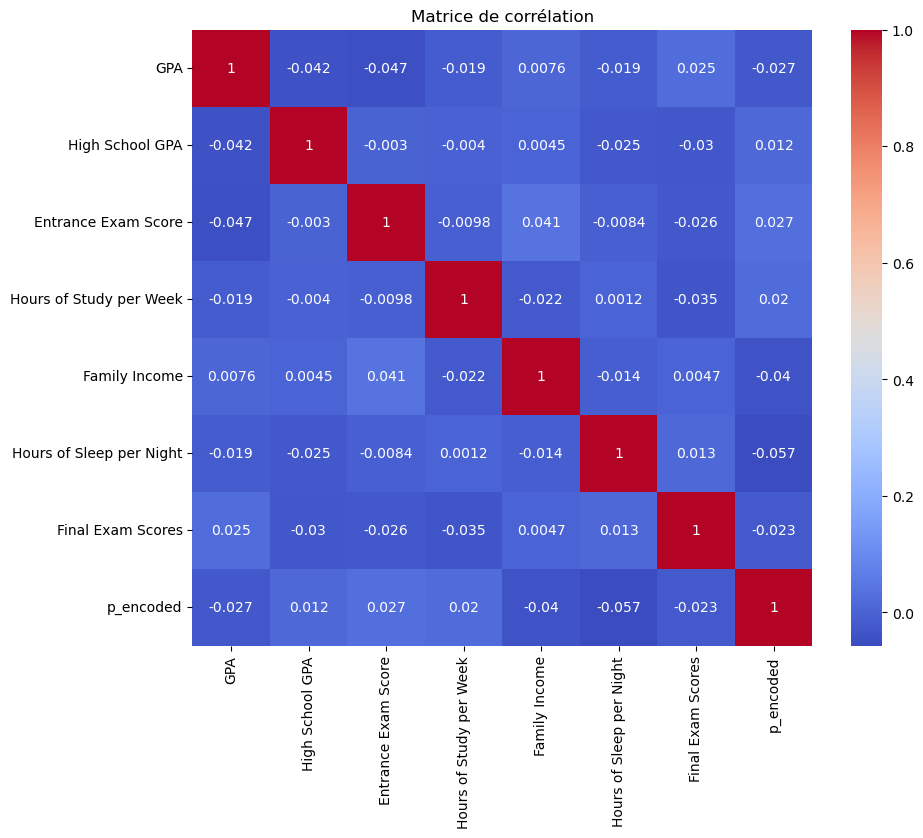
\includegraphics[width=0.9\textwidth]{../figures/corr1}
	\caption{}
	\label{fig:corr1}
\end{figure}

\vspace{0.5cm}
\textbf{Choix des variables explicatives (X) :} \\
Parmi les variables ci-dessus, nous avons sélectionné les variables suivantes :
\begin{itemize}
	\item GPA
	\item Final Exam Scores
	\item Gender
	\item Parental Education Level
	\item Family Income
	\item Hours of Study per Week
\end{itemize}

\vspace{0.3cm}
\textbf{Variable cible (Y) :} \\
La variable cible est \textbf{Performance} ou \textbf{P\_encoded}. Elle correspond à environ 70\% de notre objectif d'étude, car elle représente la performance des étudiants mais pas exactement la classification.

\section{Visualisation des données du dataset principal}

\section{Analyse univariée}

\subsection{GRE Score}
Pour analyser la distribution du GRE Score, nous avons utilisé un histogramme (\textbf{Figure 1.4}).

\begin{figure}[!htbp]
	\centering
	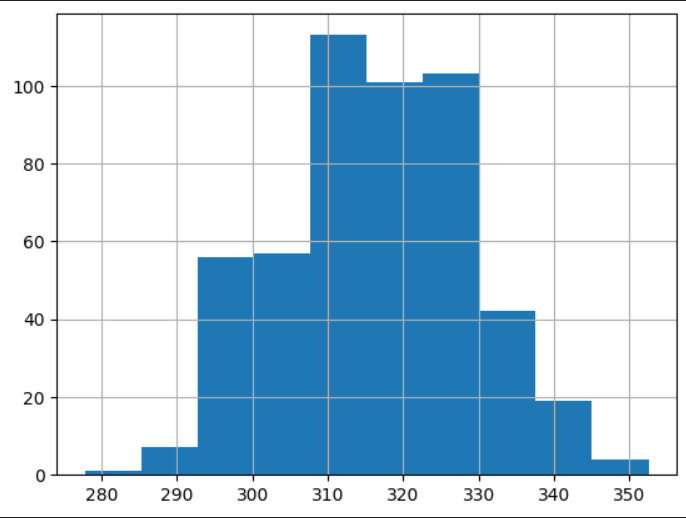
\includegraphics[width=0.9\textwidth]{../figures/hist_gre_score.png}
	\caption{Distribution du GRE Score}
	\label{fig:hist_gre_score}
\end{figure}

La majorité des scores GRE se situe entre 300 et 335, montrant une répartition homogène avec une concentration autour de scores élevés.

\subsection{CGPA}
Distribution du CGPA (\textbf{Figure 1.5}).

\begin{figure}[!htbp]
	\centering
	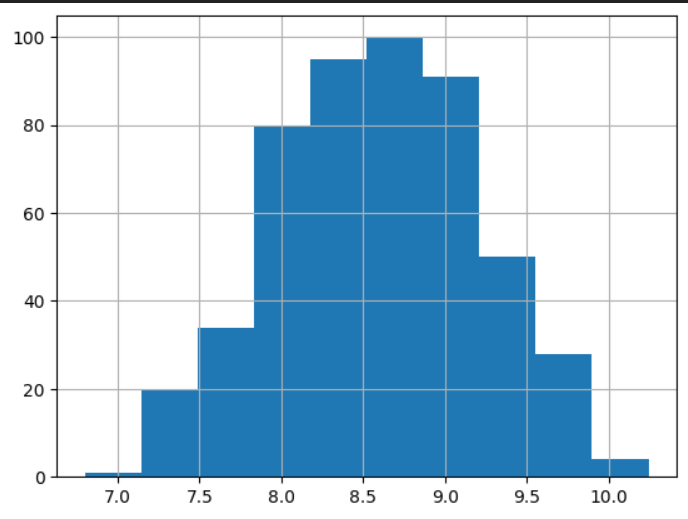
\includegraphics[width=0.9\textwidth]{../figures/hist_cgpa.png}
	\caption{Distribution du CGPA}
	\label{fig:hist_cgpa}
\end{figure}

La majorité des CGPA sont entre 8.0 et 9.5, peu de candidats en dessous de 7.5.

\subsection{TOEFL Score}
Distribution du TOEFL Score (\textbf{Figure 1.6}).

\begin{figure}[!htbp]
	\centering
	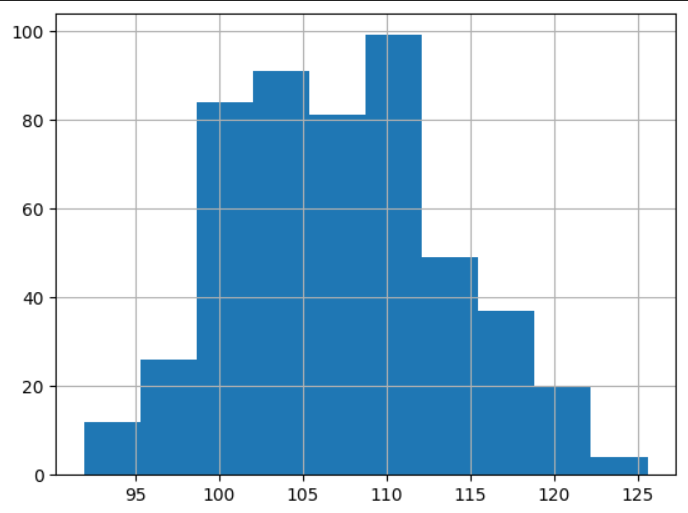
\includegraphics[width=0.9\textwidth]{../figures/hist_toefl_score.png}
	\caption{Distribution du TOEFL Score}
	\label{fig:hist_toefl_score}
\end{figure}

Les scores se concentrent entre 100 et 110, avec quelques candidats dépassant 115.

\subsection{University Rating}
Distribution de University Rating (\textbf{Figure 1.7}).

\begin{figure}[!htbp]
	\centering
	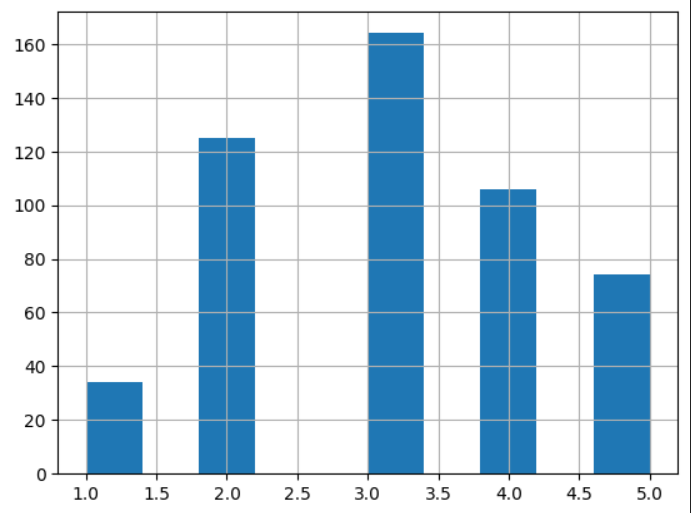
\includegraphics[width=0.9\textwidth]{../figures/hist_university_rating.png}
	\caption{Distribution de l'évaluation des universités}
	\label{fig:hist_university_rating}
\end{figure}

Les notes sont principalement entre 2 et 4.

\subsection{Research}
Répartition des étudiants selon expérience de recherche (\textbf{Figure 1.8}).

\begin{figure}[!htbp]
	\centering
	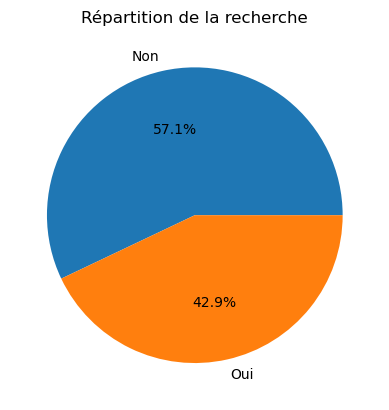
\includegraphics[width=0.9\textwidth]{../figures/pie.png}
	\caption{Répartition des candidats selon l’expérience de recherche}
	\label{fig:pie_research}
\end{figure}

57.1\% ont une expérience de recherche contre 42.9\% qui n’en ont pas.

\subsection{Chance of Admit}
Distribution de la probabilité d’admission (\textbf{Figure 1.9}).

\begin{figure}[!htbp]
	\centering
	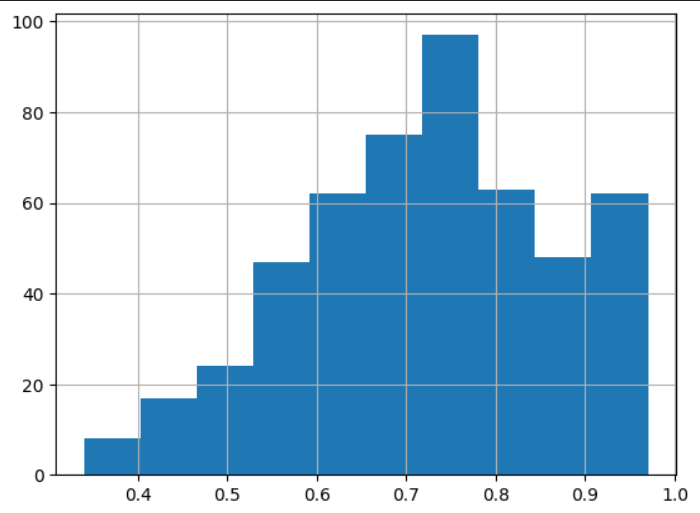
\includegraphics[width=0.9\textwidth]{../figures/hist_chance_admit.png}
	\caption{Distribution de la probabilité d’admission}
	\label{fig:hist_chance_admit}
\end{figure}

La majorité des valeurs se situe entre 0.6 et 0.8, avec une deuxième concentration entre 0.8 et 0.9.

\section{Analyse bivariée}

\subsection{GRE Score vs Chance of Admit}
Nuage de points (\textbf{Figure 1.10}).

\begin{figure}[!htbp]
	\centering
	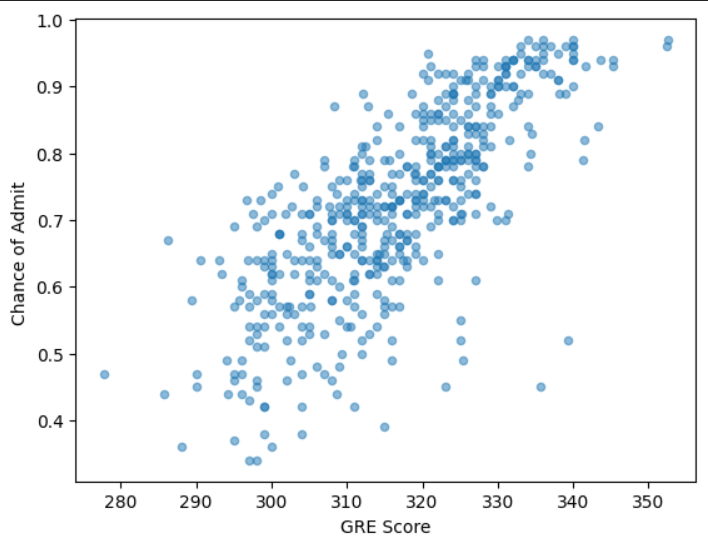
\includegraphics[width=0.9\textwidth]{../figures/scatter_gre_admit.png}
	\caption{Relation entre GRE Score et Chance of Admit}
	\label{fig:scatter_gre_admit}
\end{figure}

Relation croissante : GRE > 320 → plus de chances d’admission.

\subsection{CGPA vs Chance of Admit}
Nuage de points (\textbf{Figure 1.11}).

\begin{figure}[!htbp]
	\centering
	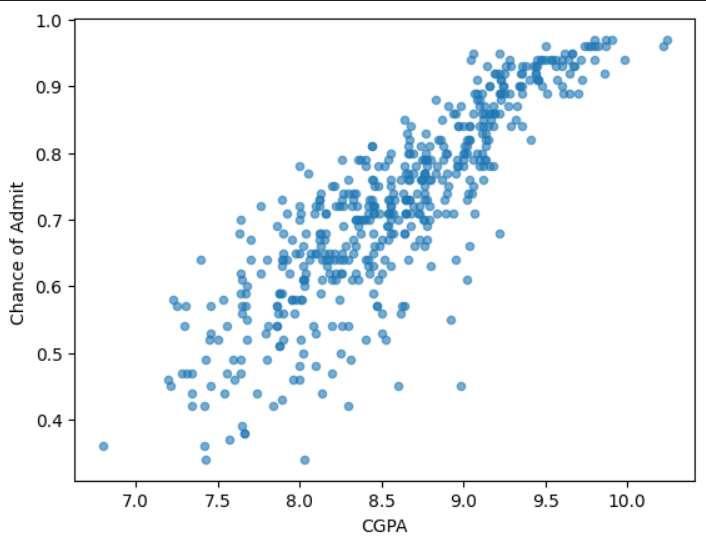
\includegraphics[width=0.9\textwidth]{../figures/scatter_cgpa_admit.png}
	\caption{Relation entre CGPA et Chance of Admit}
	\label{fig:scatter_cgpa_admit}
\end{figure}

Forte corrélation positive : CGPA élevé → chance d’admission élevée.

\subsection{TOEFL Score vs Chance of Admit}
Nuage de points (\textbf{Figure 1.12}).

\begin{figure}[!htbp]
	\centering
	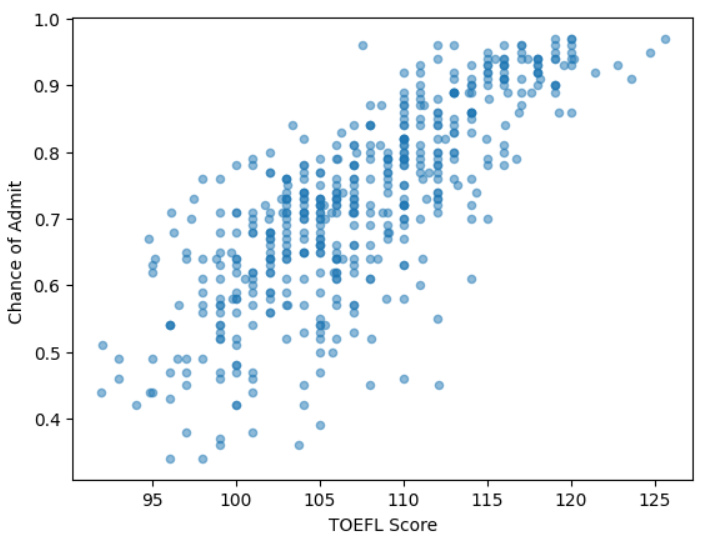
\includegraphics[width=0.9\textwidth]{../figures/scatter_toefl_admit.png}
	\caption{Relation entre TOEFL Score et Chance of Admit}
	\label{fig:scatter_toefl_admit}
\end{figure}

Tendance similaire : TOEFL élevé → chance d’admission élevée. Lignes verticales indiquent plusieurs étudiants ayant le même score.

\subsection{Chance of Admit par expérience de recherche}
Boîte à moustaches (\textbf{Figure 1.13}).

\begin{figure}[!htbp]
	\centering
	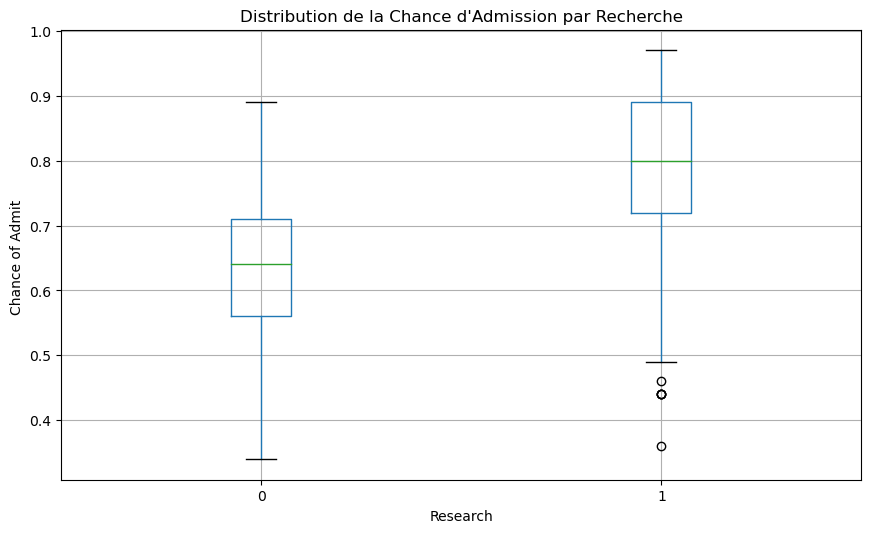
\includegraphics[width=0.9\textwidth]{../figures/distribution_par_search.png}
	\caption{Chance of Admit en fonction de l’expérience de recherche}
	\label{fig:boxplot_research_admit}
\end{figure}

Différence nette :
\begin{itemize}
	\item Sans recherche (0) : médiane ≈ 0.65
	\item Avec recherche (1) : médiane ≈ 0.8, 3ème quartile ≈ 0.89
\end{itemize}

\subsection{Distribution du TOEFL selon University Rating}
\begin{figure}[!htbp]
	\centering
	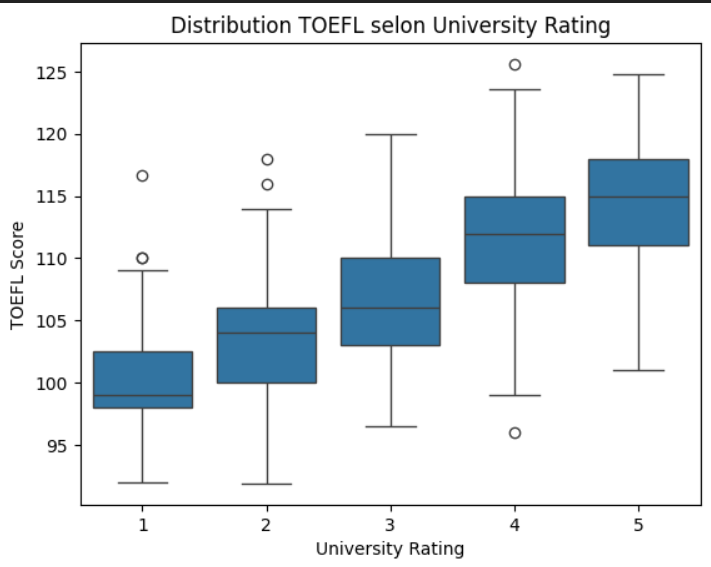
\includegraphics[width=0.9\textwidth]{../figures/TU.png}
	\caption{Distribution du TOEFL selon University Rating}
	\label{fig:TOEFLtoUR}
\end{figure}

Universités mieux classées (4-5) → scores TOEFL plus élevés, corrélation positive.

\subsection{Nombre de candidats selon expérience de recherche}
Histogramme (\textbf{Figure 1.15}).

\begin{figure}[!htbp]
	\centering
	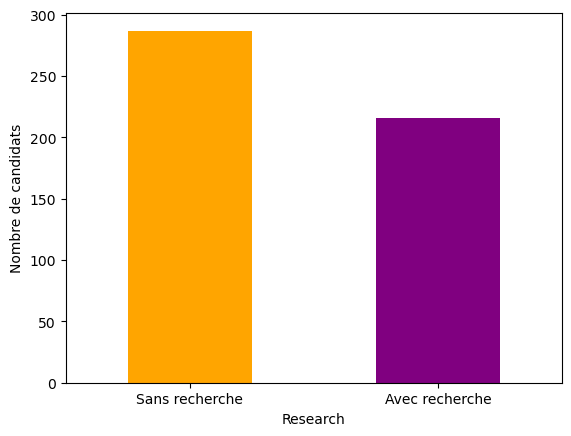
\includegraphics[width=0.9\textwidth]{../figures/nbr_selon_search.png}
	\caption{Répartition des candidats avec ou sans expérience de recherche}
	\label{fig:bar_research_counts}
\end{figure}

Environ 250-300 candidats sans expérience et 200-250 avec expérience.

\section{Conclusion de l'exploration}

Cette exploration met en évidence :
\begin{itemize}
	\item Corrélation positive entre GRE, TOEFL, CGPA et chance d’admission ;
	\item Influence de l’expérience de recherche sur la probabilité d’admission ;
	\item Distribution relativement équilibrée avec certaines zones de concentration.
\end{itemize}

Ces observations guideront les choix de modélisation dans les sections suivantes.
